\subsection{Неравенство Клаузиуса. Закон возрастания энтропии (с примерами).}
\subsubsection*{Неравенство Клаузиуса}
Из первой и второй теоремы Карно следует следующие неравенство:
\begin{align} \label{35.1}
	\frac{Q_1 - Q_2'}{Q_1} \leqslant \frac{T_1 - T_2}{T_1}
\end{align}

В данном случае знак в неравенстве обоснован тем, что при равенстве ($=$) он соответствует случаю описания \textit{обратимой} тепловой машины, а знак меньше ($<$) - описанию \textit{необратимой тепловой машины}.

Формулу \eqref{35.1} можно преобразовать к виду:
\begin{align} \label{35.2}
	\frac{T_2}{T_1} \leqslant \frac{Q_2'}{Q_1}
\end{align}

В свою очередь выражение \eqref{35.2} дает:
\begin{align} \label{35.3}
	\frac{Q_1}{T_1} - \frac{Q_2'}{T_2} \leqslant 0
\end{align}

Если полученное выражение записать через количество теплоты, подводимой к рабочему телу от нагревателя  и холодильника , то оно примет окончательную форму:
\begin{align} \label{35.4}
	\boxed{\frac{Q_1}{T_1} + \frac{Q_2}{T_2} \leqslant 0}
\end{align}

При переходе к бесконечному числу тепловых резервуаров, с которыми рабочее тело тепловой машины обменивается теплотой:
\begin{align} \label{35.5}
	\boxed{\oint \frac{d Q}{T} \leqslant 0}
\end{align}

\subsubsection*{Закон возрастания энтропии}

\begin{figure}[H]
	\centering
	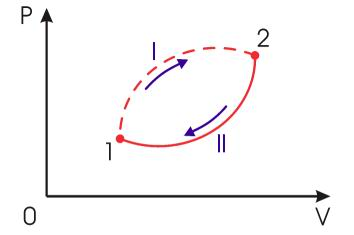
\includegraphics[width=0.7\linewidth]{image/Rule}
	\caption{График $pV$-диаграммы, иллюстрирующий закон возрастания энтропии.
		Кривые I и II представляют разные термодинамические процессы между состояниями 1 и 2.}
	\label{fig:8}
\end{figure}

Для любого необратимого процесса в замкнутой системе энтропия возрастает,
а для обратимого процесса остается постоянной. Математически это выражается
через интеграл Клаузиуса и изменение энтропии.
\begin{align} \label{35.6}
	\int\limits_{1\,I\,2} \frac{dQ}{T} + \int\limits_{2\,II\,1} \frac{dQ}{T} < 0
	\Rightarrow
	S_2 - S_1 > \int_{1}^{2} \frac{dQ}{T}
\end{align}

Здесь интегралы представляют циклический процесс, где первый интеграл - по пути I из состояния 1 в 2, а второй - по пути II из 2 в 1. Неравенство показывает, что для необратимого процесса изменение энтропии больше, чем интеграл от приведенного тепла.

Из чего следует фундаментальное неравенство:
\begin{align} \label{35.7}
	\boxed{S_2 - S_1 \geqslant \int_{1}^{2} \frac{dQ}{T}}
\end{align}

В этом обобщенном виде неравенство объединяет оба случая: для обратимых процессов (равенство) и необратимых (строгое неравенство). $dQ$ - элементарное количество тепла, переданное системе при температуре $T$.

В тепло изолированной системе ($dU = 0$), следует запись:
\begin{align} \label{35.8}
	\boxed{S_2 - S_1 \geqslant 0}
\end{align}

\subsubsection*{Физические смыслы энтропии}
\begin{enumerate}
	\item \textbf{Энтропия (S)} мера необратимости процессов (если $\Delta S = 0$, то процесс обратим). Чем больше $\Delta S = S_2 - S_1$, тем необратимее процесс.

	Если $S_2 > S_1$, то процесс $1 \to 2$ возможен, а $2 \to 1$ нет, так как энтрапия не может возрастать.

	Второй принцип термодинамики играет роль директора -- определяет направление протекающих процессов. В замкнутой системе при достижении системой термодинамического равновесия энтропия достигает максимального значения.
	\item \textbf{Энтропия (S)} -- мера близости системы и состояния термодинамического равновесия.
	\item \textbf{Энтропия (S)} -- мера качества тепловой энергии.

	В замкнутой системе внутренняя энергия постоянна.
	\item \textbf{Энтропия (S)} -- мера вероятности макро состояния. Чем выше $S$, тем более вероятно состояние.
	\item \textbf{Энтропия (S)} -- мера беспорядка (хаоса) в системе. Чем более хаотично, тем более вероятно.
\end{enumerate}